\documentclass{article}
\usepackage{tikz, comment}
\usepackage{pifont}
\usepackage{fontspec}
\usetikzlibrary{arrows, decorations.markings, decorations.pathreplacing}
\begin{comment}
:Title: Not defined yet
:Slug: No name yet

Description Here.........
\end{comment}
\begin{document}\centering 

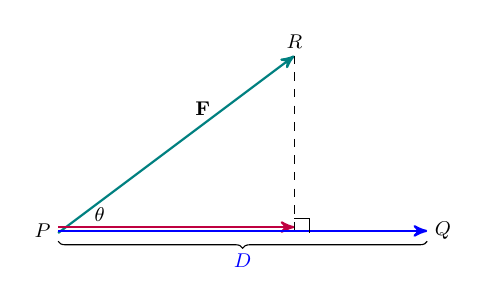
\begin{tikzpicture}[>=latex,xscale=.5*0.75, yscale=.5*0.75][font=\sf\small] 

\draw[teal, thick, ->, >=stealth'] (0, 0) -- (8, 6) node[black, left, midway, pos=0.7, xshift=-2, yshift=0, scale=0.8]{${\bf F}$}node[black, above, scale=0.8]{$R$};

\draw[purple, thick, ->, >=stealth'] (0, 0.2) -- (8, 0.2);
\draw[blue, thick, ->, >=stealth', yshift=2] (0, 0) node[black, left, scale = 0.8] {$P$}-- (12.5, 0) node[black, right, scale = 0.8] {$Q$};

\draw[dashed] (8, 6)--(8, 0);

\draw ({8+0.5}, 0)--++(0, 0.5)--++(-0.5, 0); 

\node[xshift = 15, yshift = 6.75, scale=0.8] at (0, 0) {$\theta$};

\draw [decoration={brace,raise=3, mirror},decorate, xshift=0] 
({0},{0})--({12.5},{0})node[blue, below, midway, pos=0.5, xshift=0, yshift=-5, scale=0.8]{$D$};

\end{tikzpicture}
\end{document}